\chapter{\label{chap:resultados}Resultados}

Após a avaliação da aplicação, os resultados foram compilados em duas categorias: os resultados referentes às tarefas e os resultados referentes ao questionário aplicado. Para a avaliação e validação da aplicação, participaram dos testes um avaliador com deficiência visual e cinco avaliadores sem deficiência. Estes compuseram a avaliação justamente para a comparação dos resultados entre os possíveis usuários finais do sistema. Os dados, bem como sua análise, serão apresentados nas próximas seções.

\section{Tarefas}

O teste efetuado junto ao avaliador com deficiência visual trouxe, de modo geral, bons resultados. Ao ser questionado sobre o fluxo da aplicação, em oito dos nove casos o entrevistado considerou o caminho apresentado pela aplicação condizente com o esperado, discordando, apenas, durante o uso do sistema de buscas (tarefa 4), onde o avaliador apresentou certa dificuldade. Neste caso, a aplicação não apresentava uma lista de sugestões de restaurantes e o usuário inferiu que deveria digitar o nome do local para realizar a busca. Ou seja, além de apresentar problemas com a falta de um sistema de sugestões, o usuário também não estava ciente que havia um botão de \emph{busca por voz} disposto na interface. Sendo assim, esta tarefa teve duração de doze minutos em sua primeira execução. Após ser informado que o sistema dispunha de interação por voz, a tarefa foi executada novamente, tendo duração de um minuto. Apesar disso, em sua grande maioria, o avaliador julgou o tempo de execução das tarefas adequado.
%Com o resultado desta análise, foram então implementadas sugestões de restaurantes para o sistema de busca. 
% Normalmente, o usuário navegava pela tela explorando todos seus elementos e, então, selecionava a opção desejada, levando um tempo a mais.

Já os demais participantes não apresentaram dificuldade durante a realização das tarefas. As tarefas foram cumpridas em um curto espaço de tempo, o qual variou entre um e trinta e quatro segundos. Além disso, os resultados foram, em sua maioria, positivos, e os usuários reagiram de maneira assertiva ao interagir com a aplicação. Dito isso, algumas mudanças foram sugeridas, as quais serão apresentadas na seção \ref{sec:sugestoes}. Os tempos de execução das tarefas realziadas pelos usuários sem deficiência são apresentados no gráfico a seguir:

\begin{figure}[H]
	\centering
	\caption[Tempo de execução -- Usuários sem deficiência visual]{Tempo de execução das tarefas dos usuários sem deficiência visual}
	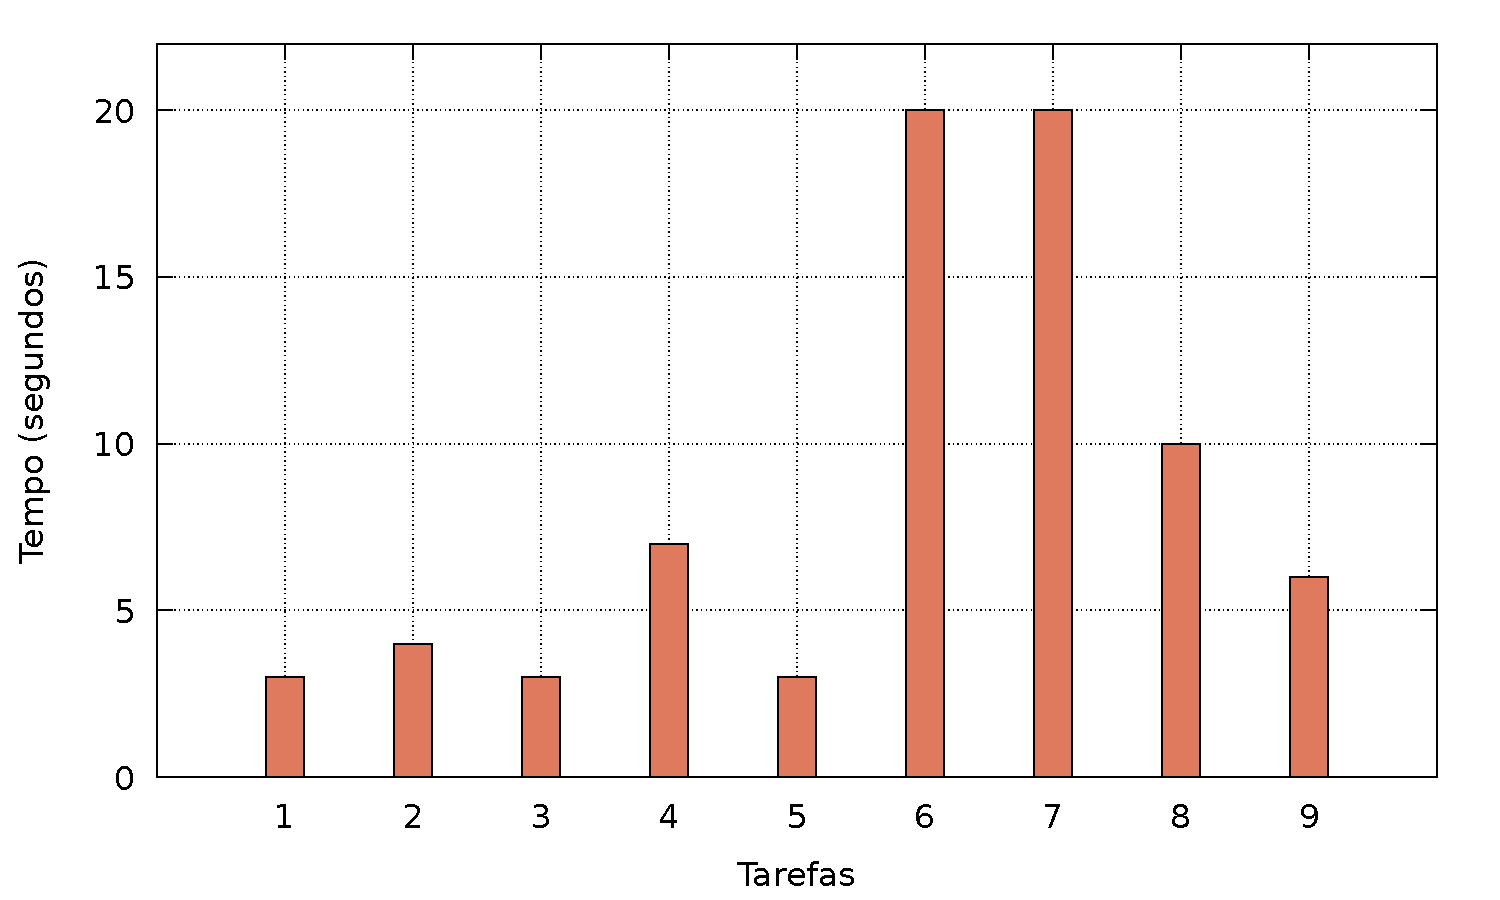
\includegraphics[width=0.8\linewidth]{./charts/tempo-sem-dv.pdf}
	\label{fig:tempo-sem-dv}
\end{figure}

Comparando o tempo gasto por estes usuários durante a realização das tarefas e o período que o avaliador com deficiência visual levou para executar as mesmas funções, nota-se uma grande diferença entre os resultados. Esta diferença pode ser observada no gráfico da Figura \ref{fig:tempo}.

\begin{figure}[H]
	\centering
	\caption[Tempo de execução -- Geral]{Tempo de execução das tarefas (geral)}
	\label{fig:tempo}
	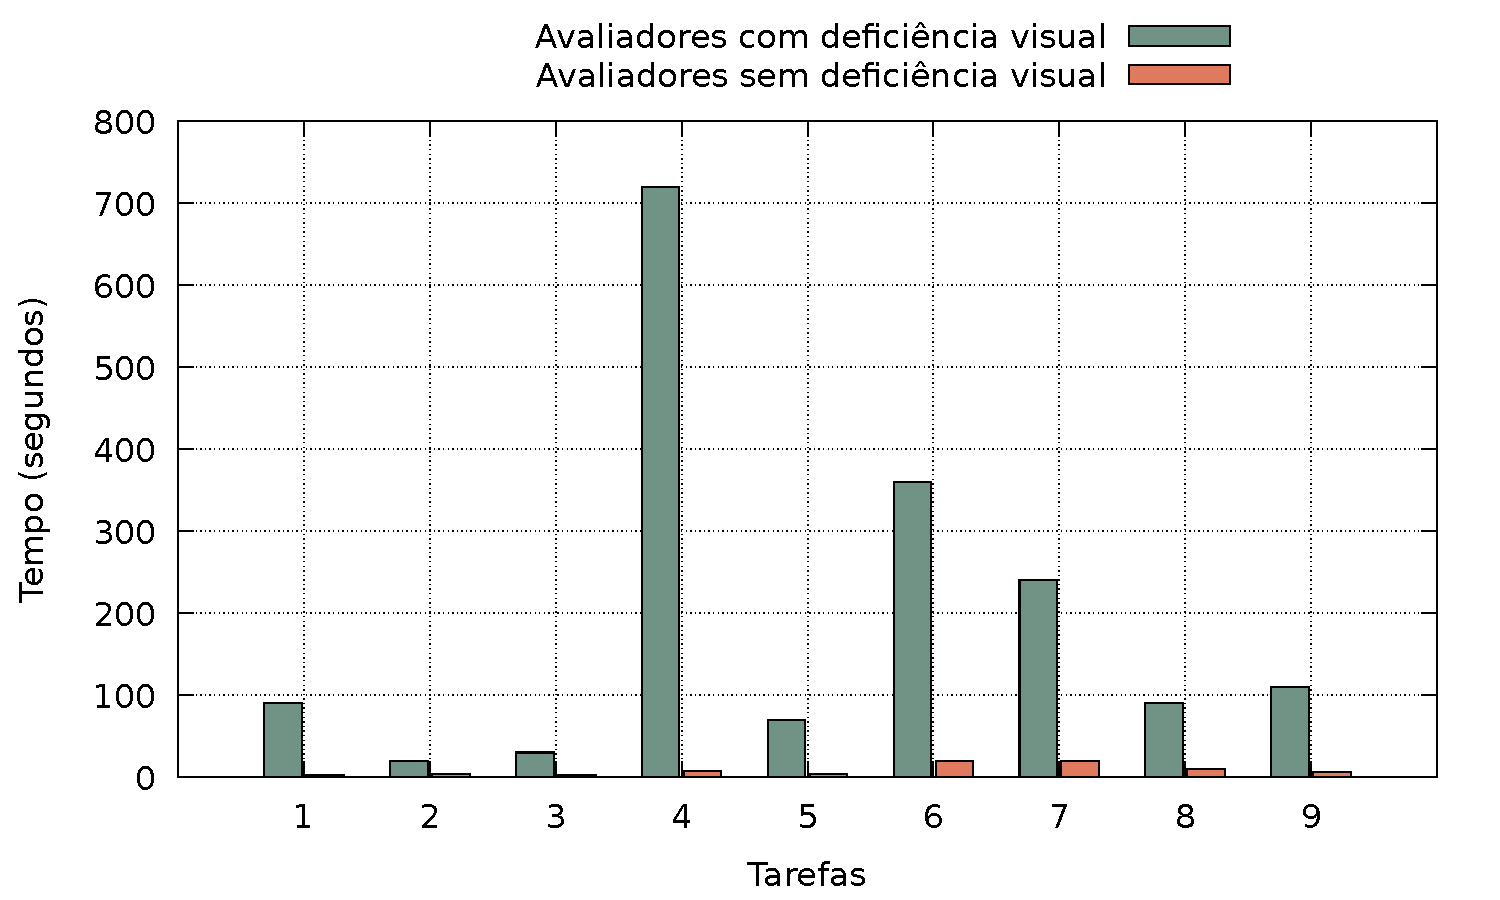
\includegraphics[width=0.8\linewidth]{./charts/tempo.pdf}
\end{figure}
Apesar do avaliador que é cego ter conseguido executar boa parte das tarefas sem grandes dificuldades, destaca-se, aqui, quão dilatado foi seu tempo de execução se comparado com o tempo dos usuários sem deficiência. Apesar de existir um sistema que proporcione acessibilidade a usuários com deficiência visual, a capacidade de interação com a aplicação através de meios visuais ainda possibilita retornos mais rápidos. Por exemplo, ao deparar-se com uma tela, um usuário sem deficiência visual tem acesso a todos os componentes dispostos nela. Já o usuário que é cego precisa navegar por toda a tela para, primeiramente, saber o que está sendo apresentado a ele. Sendo assim, os ritmos e os tempos de execução entre ambos os grupos tornam-se bastante diferentes.

\section{Questionário}

Ao avaliar a aplicação de acordo com as heurísticas de Nielsen, o avaliador que é cego manifestou aprovação em relação a maioria dos aspectos da aplicação.  As primeiras oito heurísticas e os aspectos relacionados à acessibilidade tiveram total aprovação pelo usuário. Todavia, a heurística voltada a ajuda e documentação apresentou uma aprovação mediana, uma vez que estava em fase de desenvolvimento e, consequentemente, incompleta. Dito isso, a avaliação apresentou, de modo geral, resultados favoráveis, indicando a aprovação e satisfação do avaliador.

O questionário também foi respondido pelos demais participantes do processo de avaliação. Nele, houve a predominância de respostas acima da média e, em algumas categorias, indicadores de concordância máxima pelos avaliadores. O ponto mais fraco da aplicação acabou sendo os aspectos de \emph{reconhecimento, diagnóstico e recuperação de erros}. Na maioria dos casos, os avaliadores não se depararam com erros; entretanto, no teste com um avaliador específico (avaliador \#2), foram detectadas falhas que não haviam sido tratadas durante o desenvolvimento do código, levando à parada do sistema. Sendo assim, a média final da avaliação desta heurística foi a mais baixa dentre as onze categorias do questionário.

As médias das avaliações estão dispostas nos seguintes gráficos:

\begin{figure}[H]
	\centering
	\caption[Respostas do Questionário]{Médias das respostas dos questionários separadas por tema}
	\label{fig:questionario-1}
	\subfigure[c][Avaliação -- Visibilidade do Estado do Sistema]
		{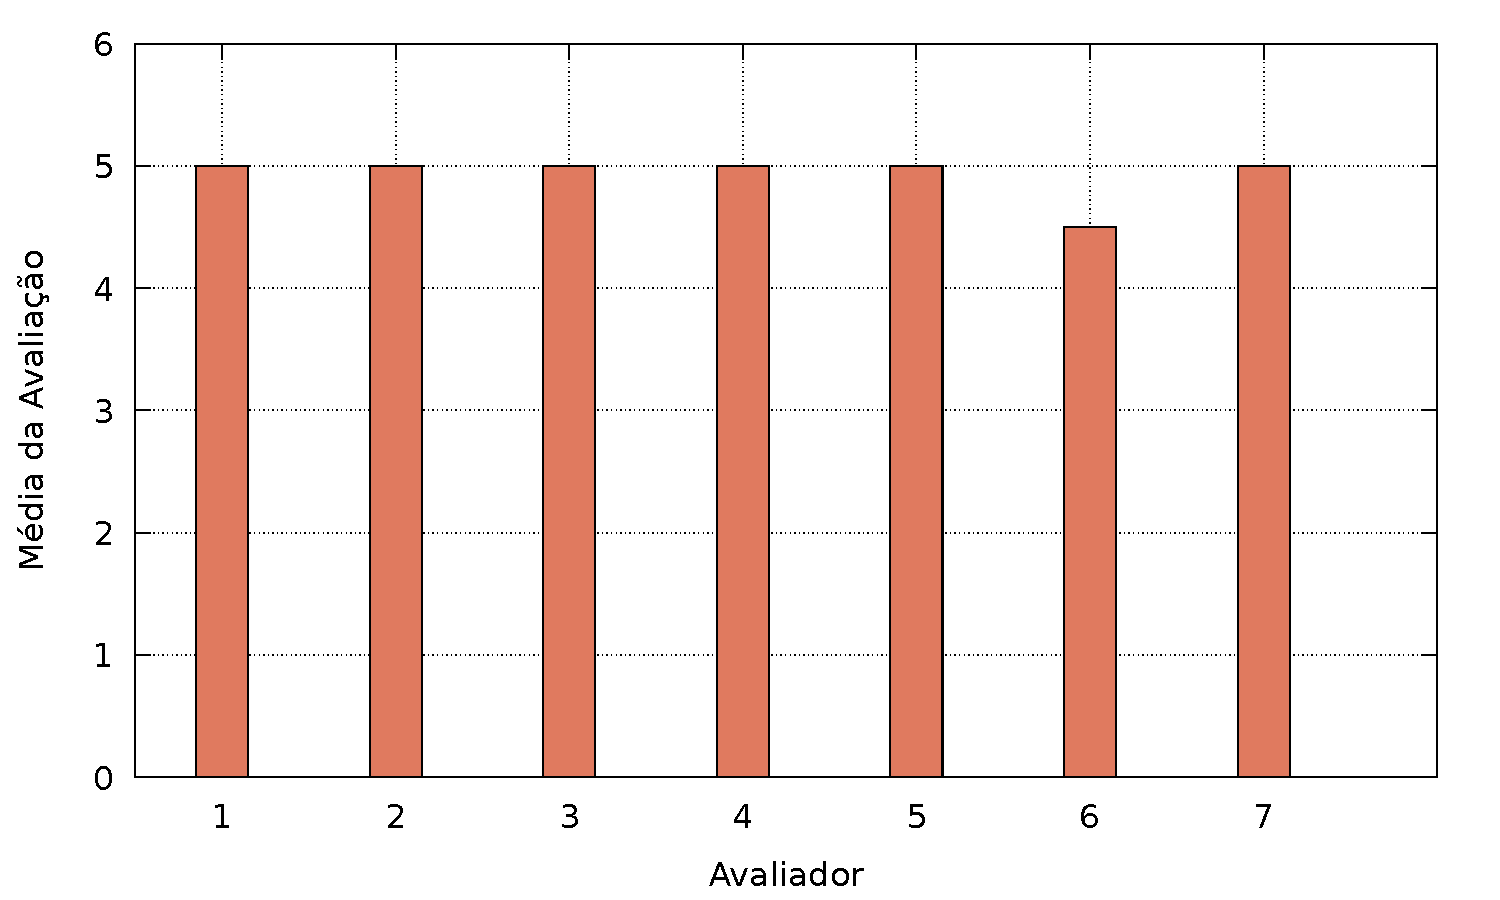
\includegraphics[width=0.45\textwidth]{charts/qt1.pdf}}
	\qquad
	\subfigure[c][Avaliação -- Correspondência entre o Sistema e o Mundo Real]
		{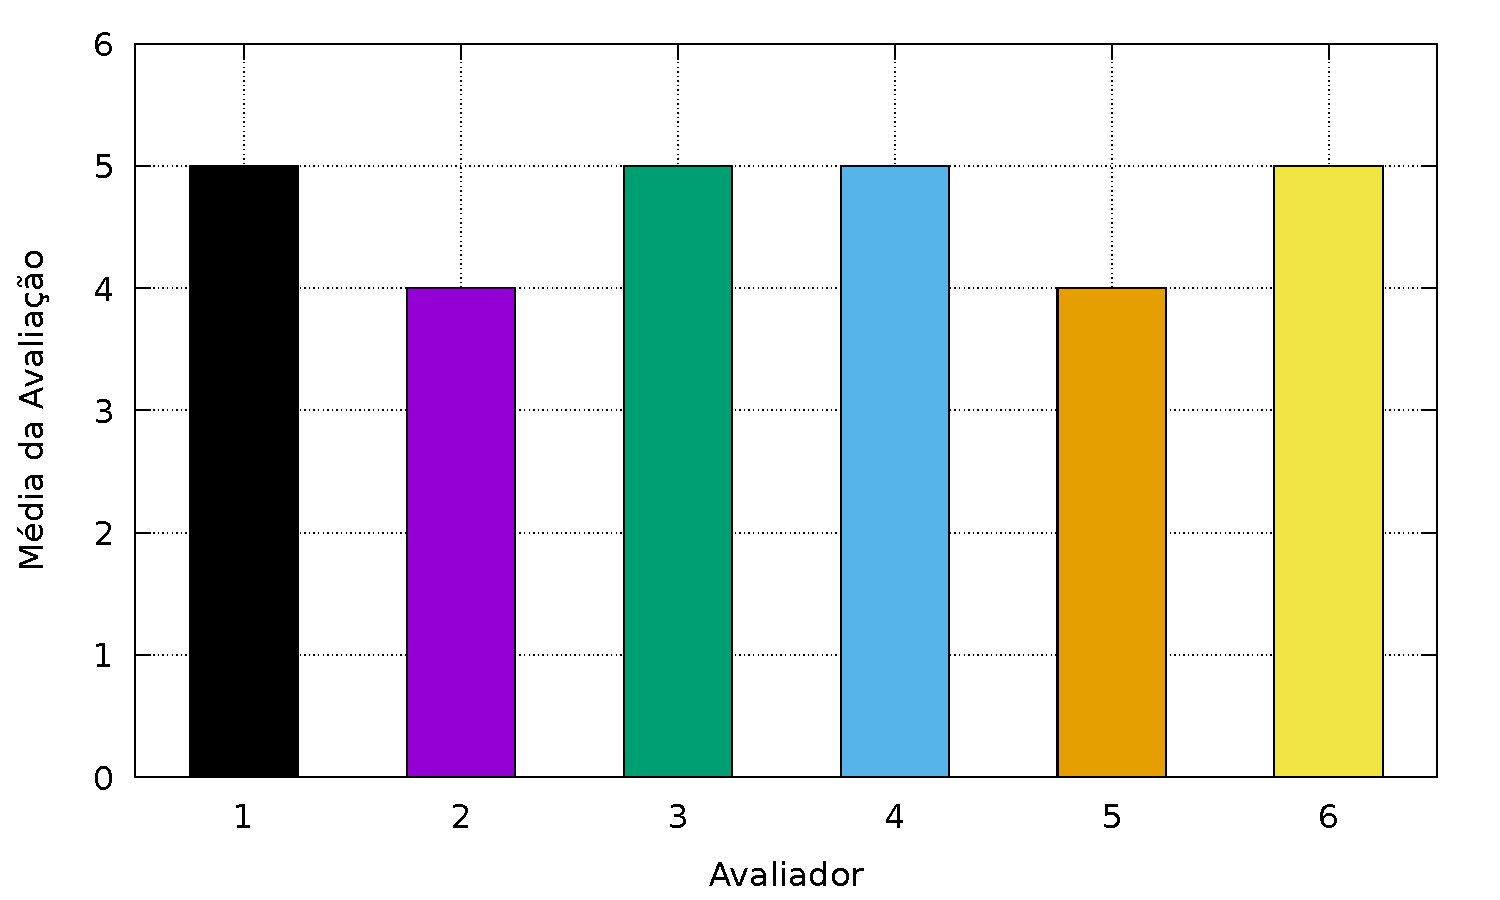
\includegraphics[width=0.45\textwidth]{charts/qt2.pdf}}
	\qquad
	\subfigure[c][Avaliação --  Controle e Liberdade do Usuário]
		{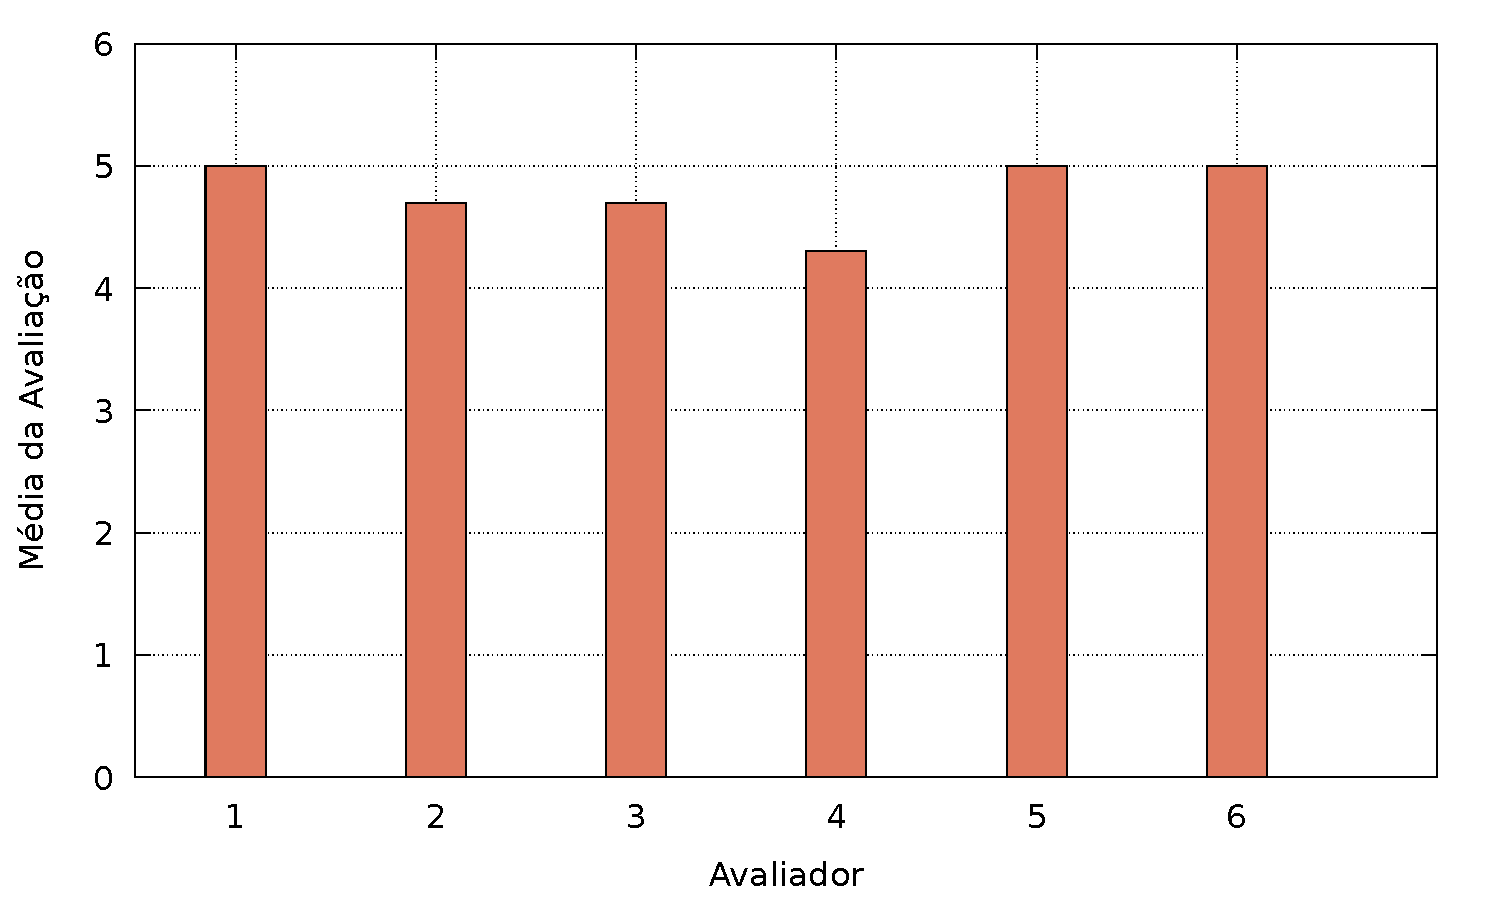
\includegraphics[width=0.45\textwidth]{charts/qt3.pdf}}
	\qquad
	\subfigure[c][Avaliação -- Consistência e Padronização]
		{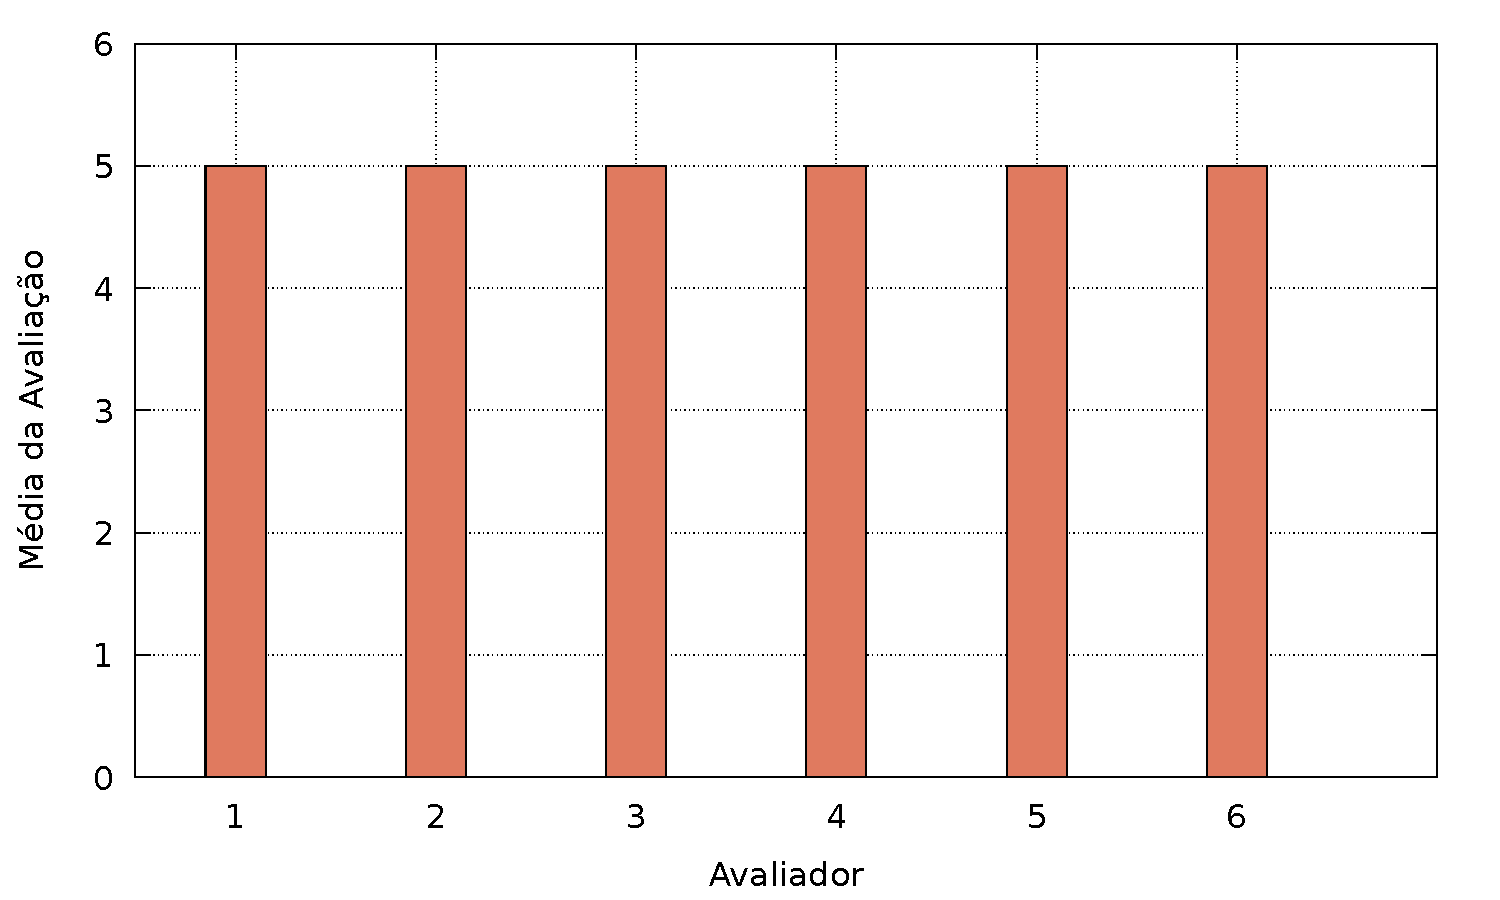
\includegraphics[width=0.45\textwidth]{charts/qt4.pdf}}
	\qquad
	\subfigure[c][Avaliação -- Prevenção de Erros]
		{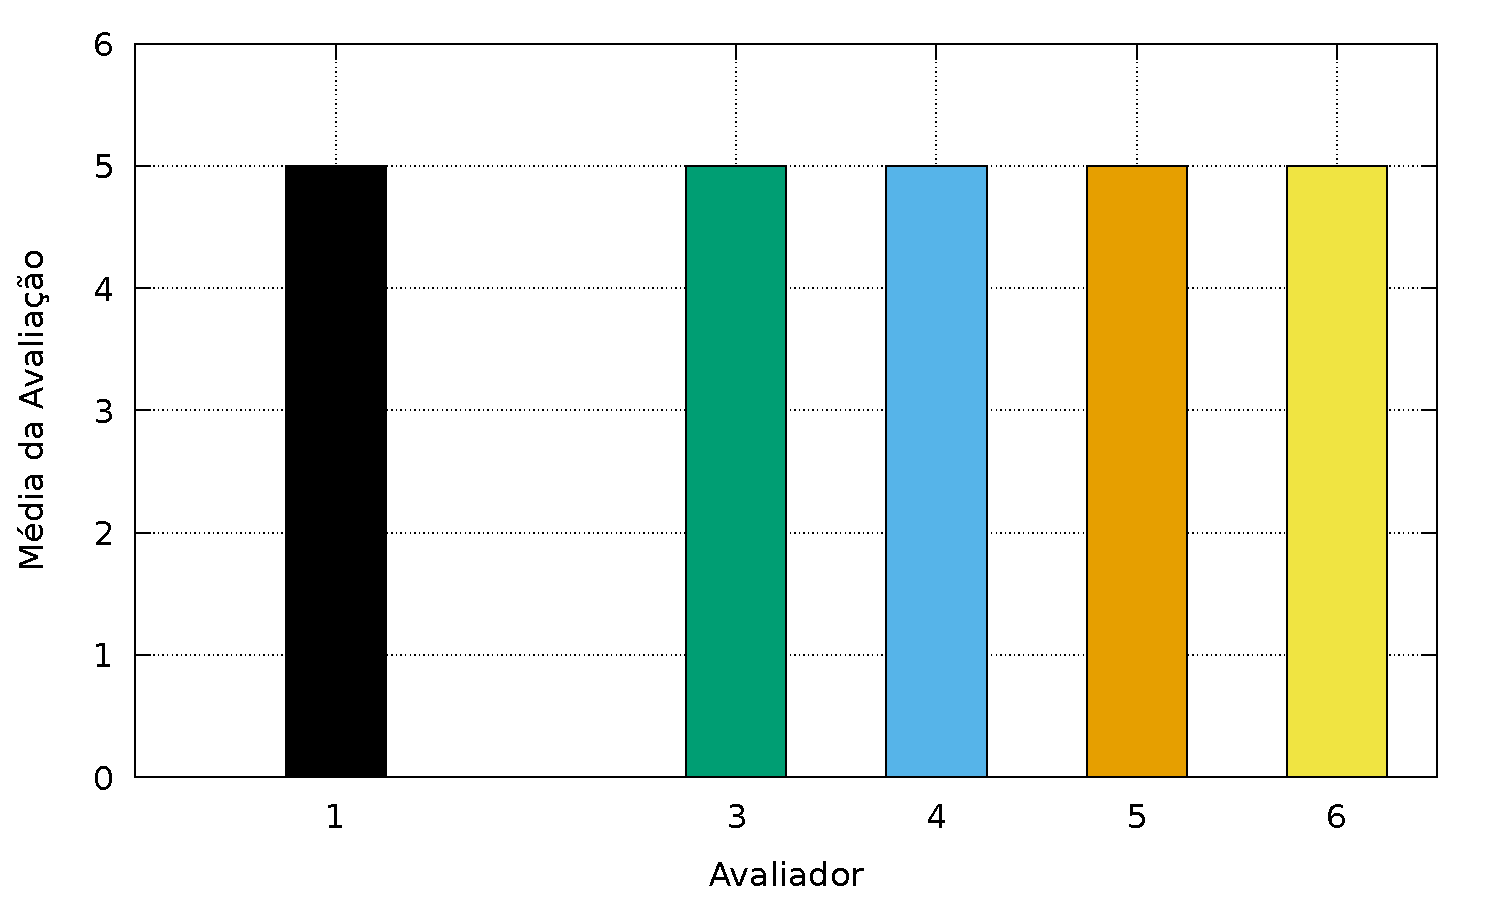
\includegraphics[width=0.45\textwidth]{charts/qt5.pdf}}
	\qquad
	\subfigure[c][Avaliação -- Reconhecimento ao Invés de Memorização]
		{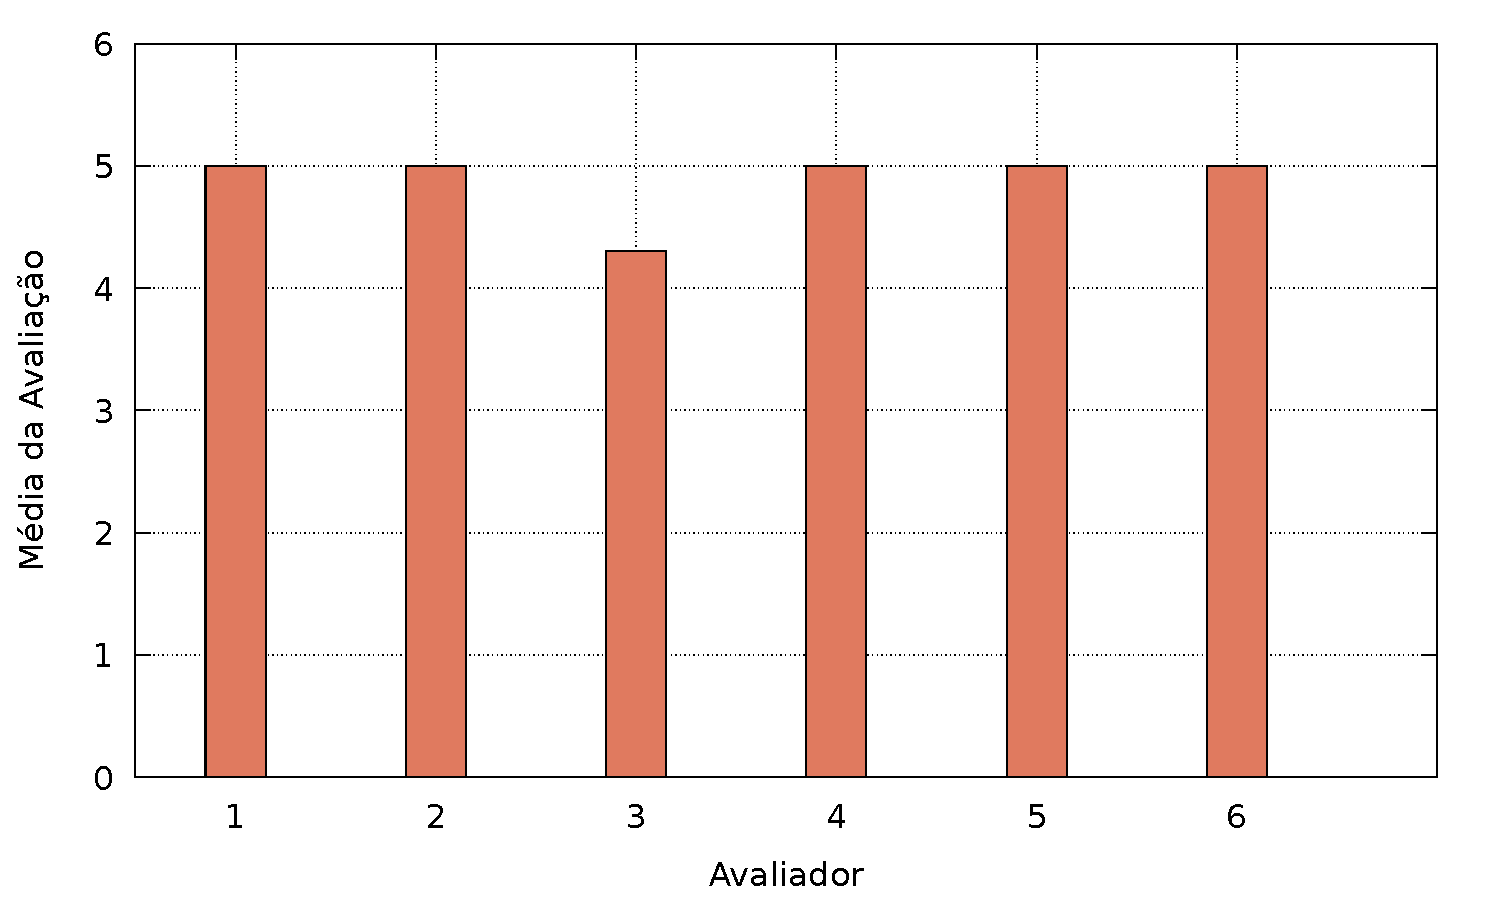
\includegraphics[width=0.45\textwidth]{charts/qt6.pdf}}
	\qquad
	\subfigure[c][Avaliação -- Flexibilidade e Eficiência de Uso]
		{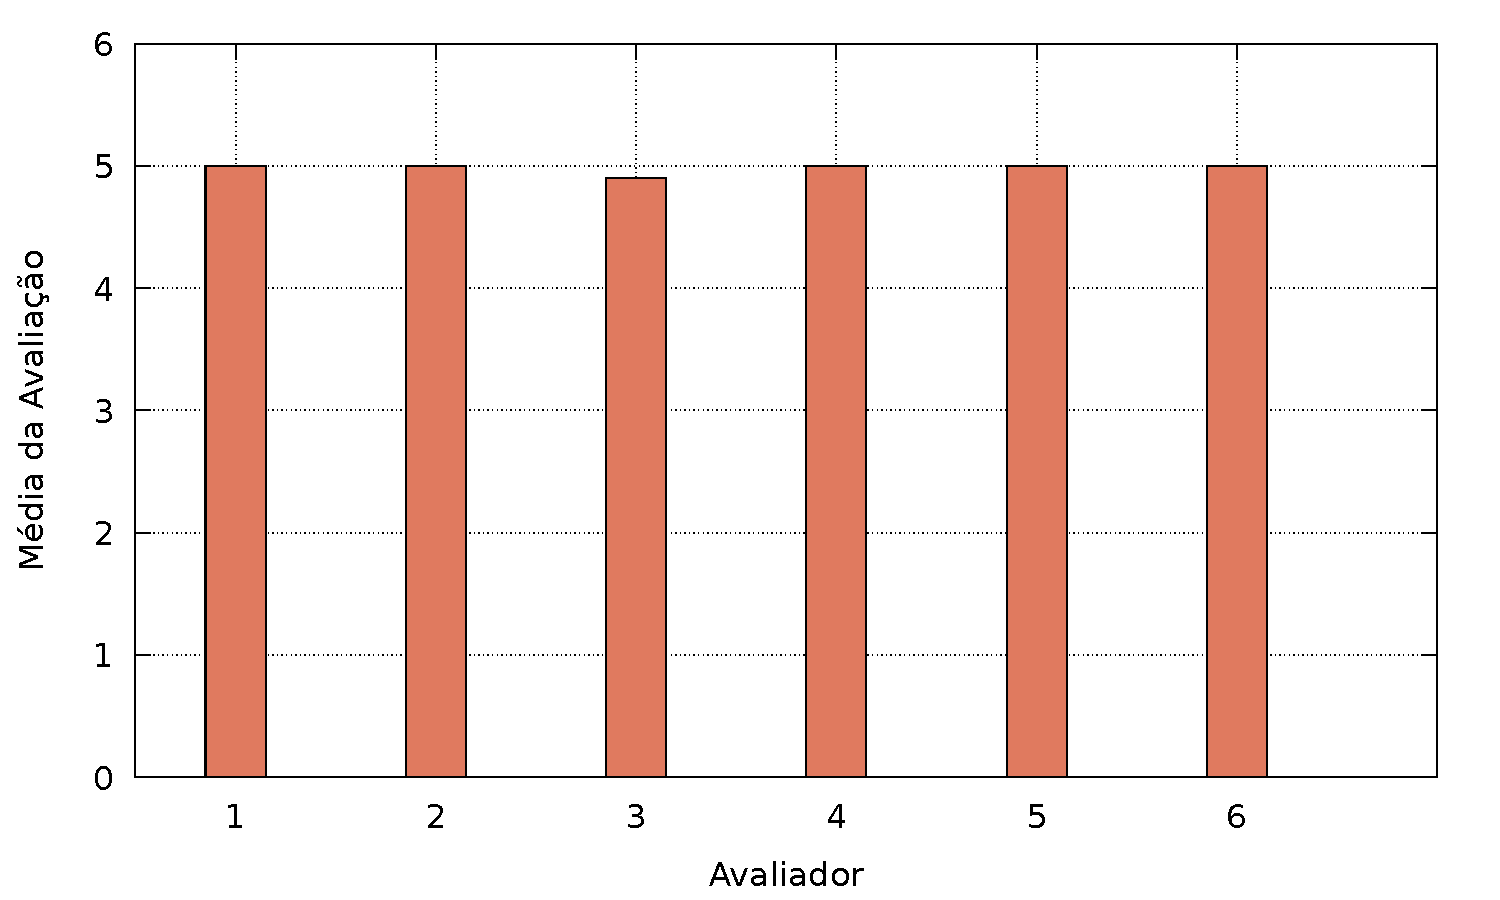
\includegraphics[width=0.45\textwidth]{charts/qt7.pdf}}
	\qquad
	\subfigure[c][Avaliação -- Projeto Estético e Minimalista]
		{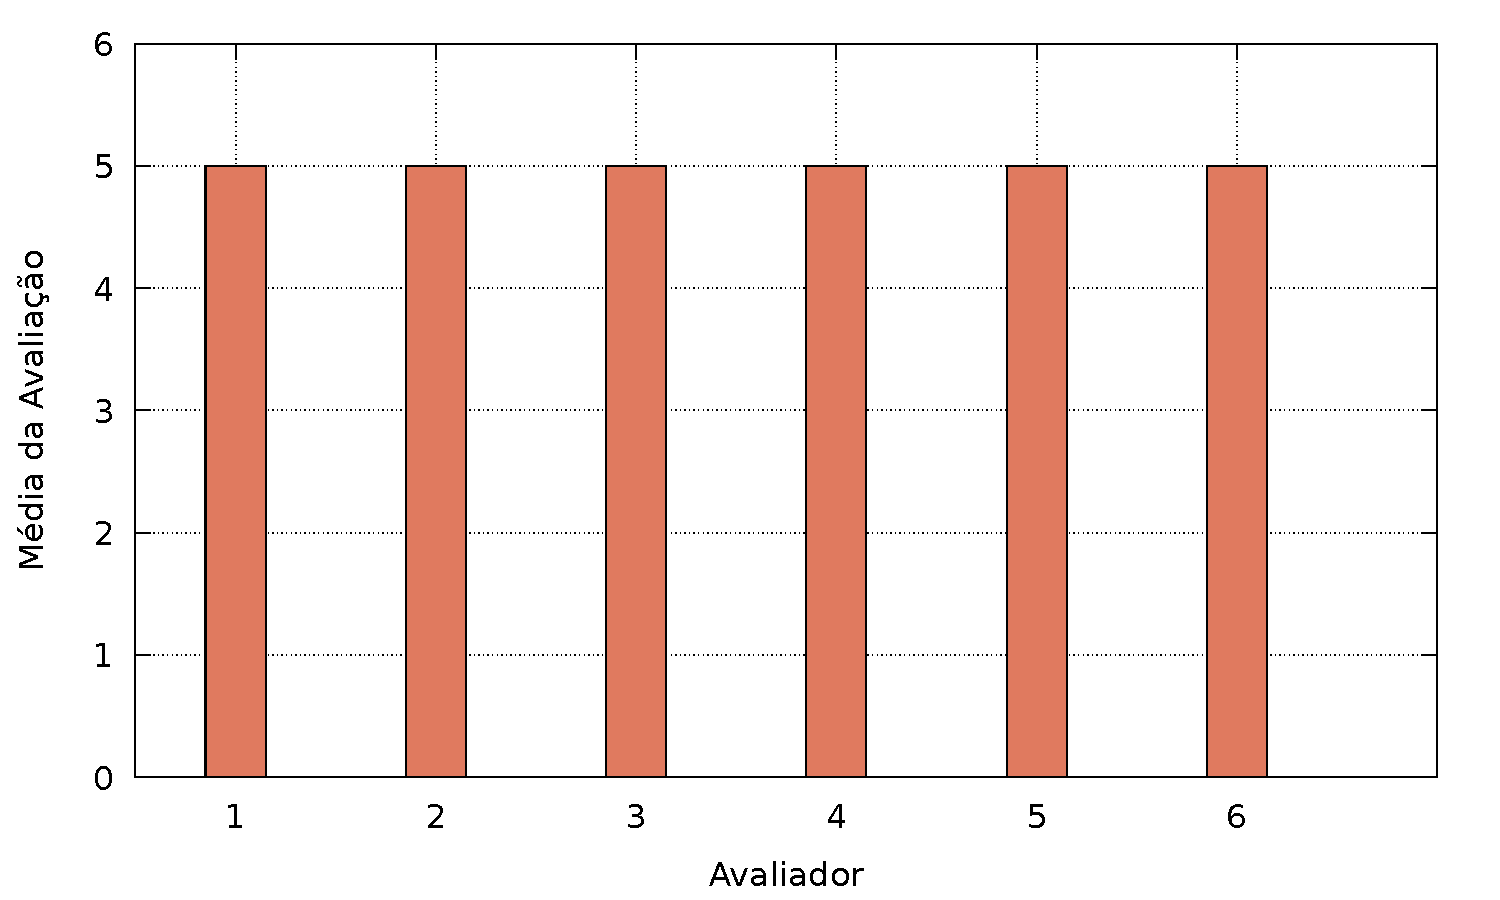
\includegraphics[width=0.45\textwidth]{charts/qt8.pdf}}
\end{figure}
	
\begin{figure}[H]\ContinuedFloat
	\centering
	\caption[]{Continuação da página anterior}
	\label{fig:questionario-2}
	\subfigure[c][Avaliação -- Reconhecimento, Diagnóstico e Recuperação de Erros]
		{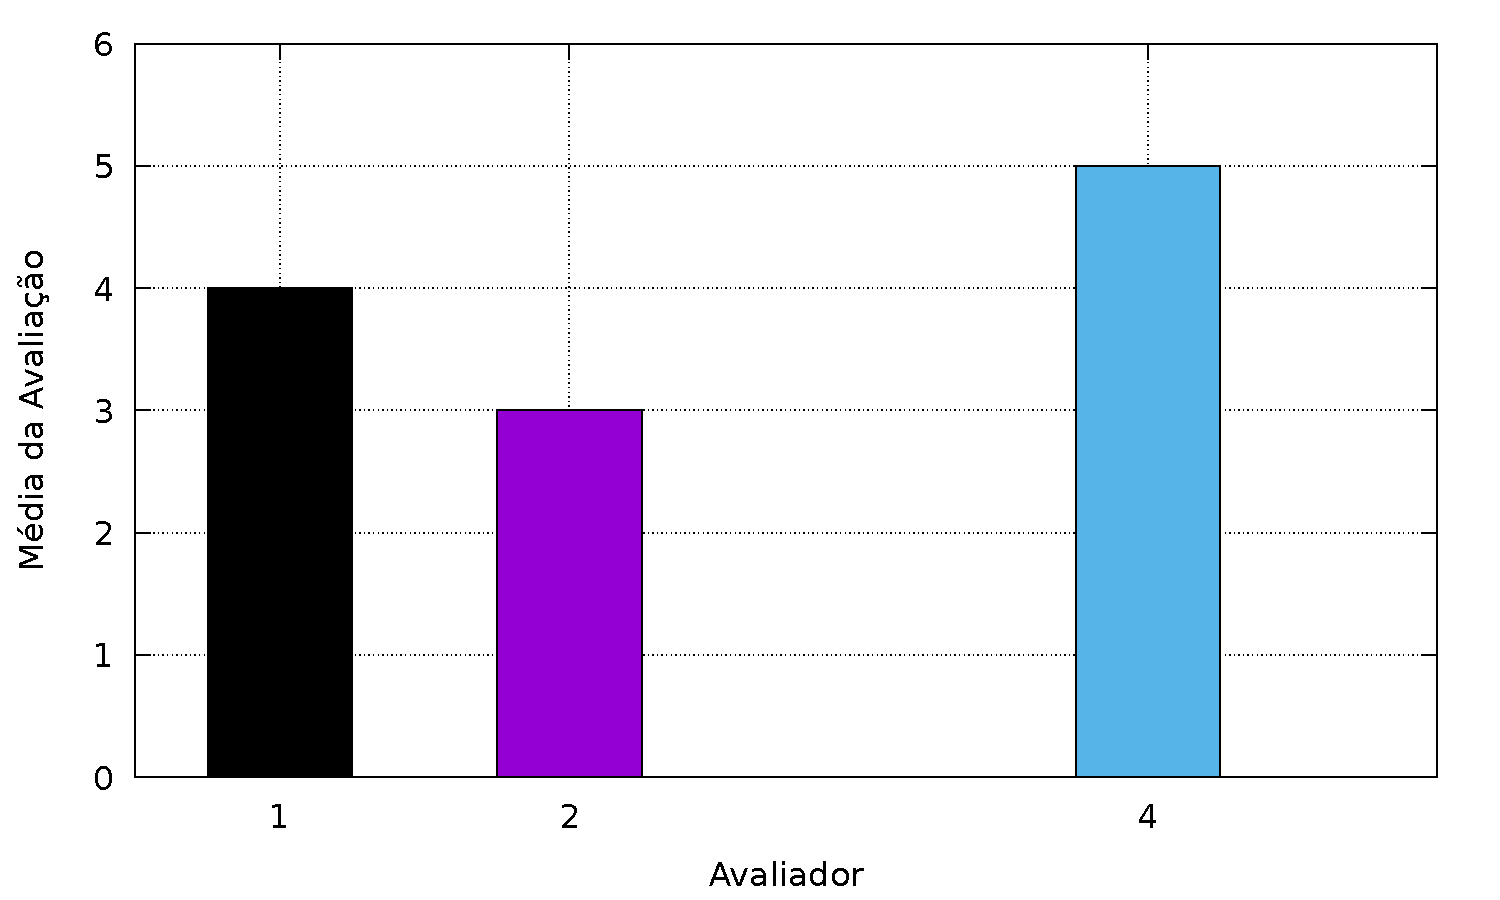
\includegraphics[width=0.45\textwidth]{charts/qt9.pdf}}
	\qquad
	\subfigure[c][Avaliação -- Ajuda e Documentação]
		{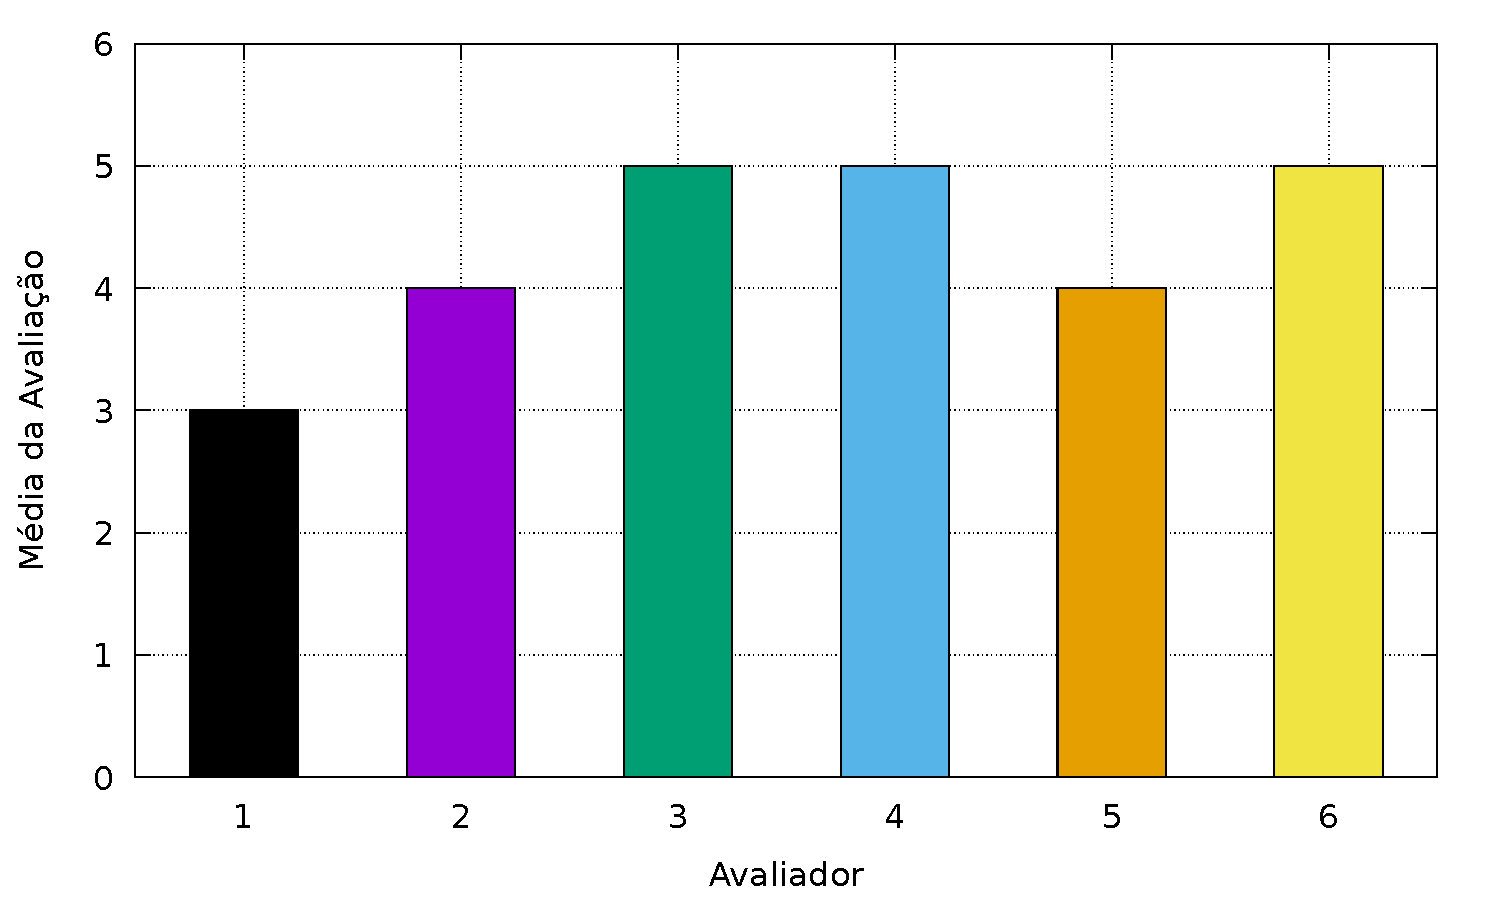
\includegraphics[width=0.45\textwidth]{charts/qt10.pdf}}
	\qquad
	\subfigure[c][Avaliação -- Acessibilidade]
		{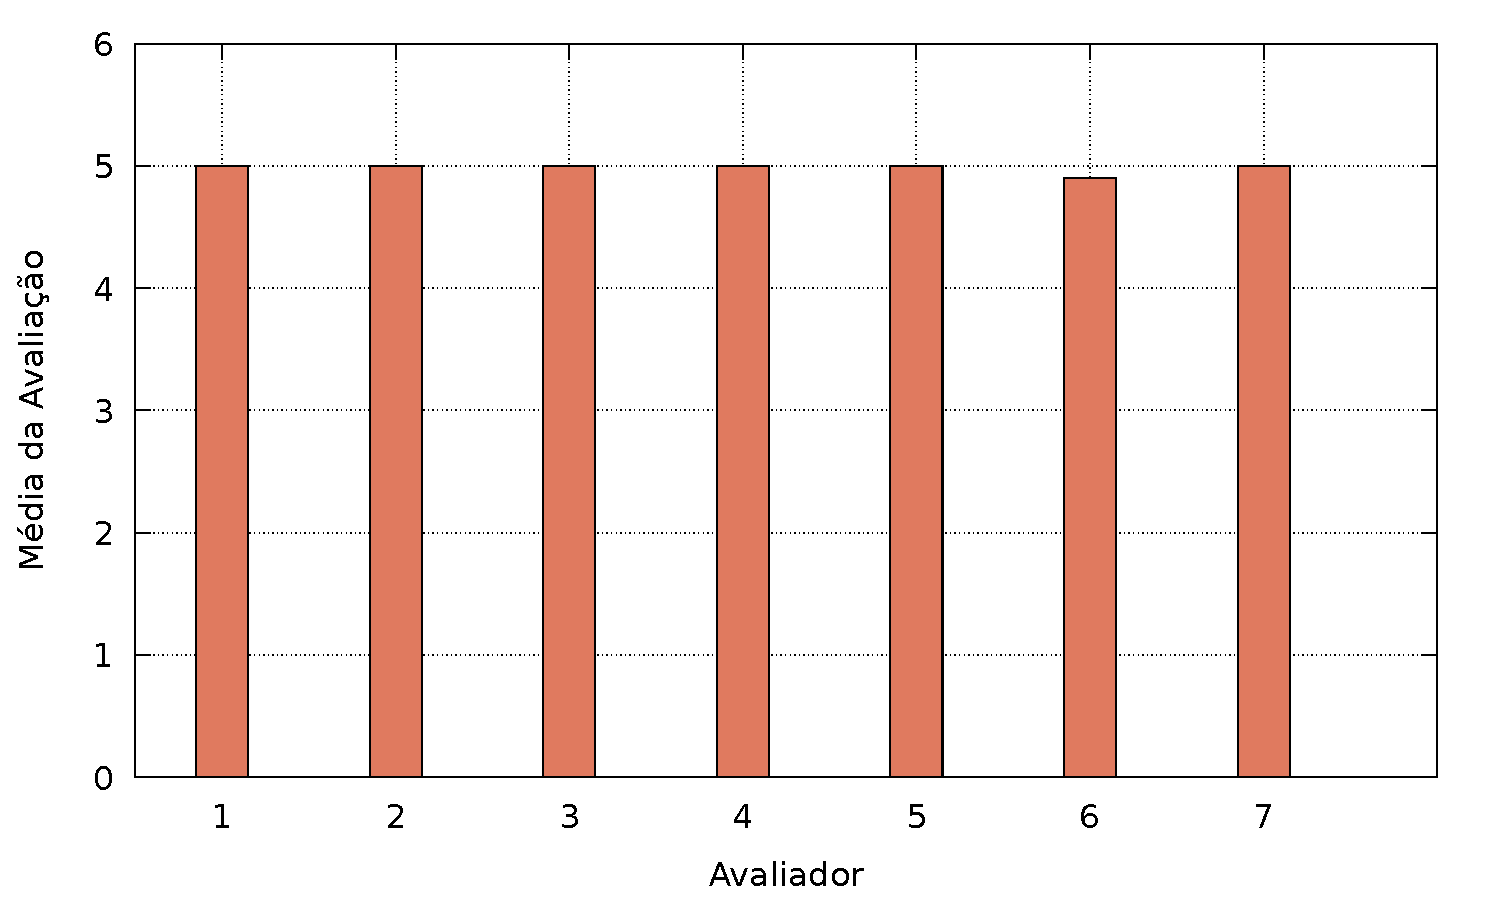
\includegraphics[width=0.45\textwidth]{charts/qt11.pdf}}	
\end{figure}

A partir dos resultados apresentados acima, contemplam-se alguns aspectos. Primeiramente, destaca-se que os fatores Consistência e Padronização (Figura \ref{fig:questionario-1}(d)), Prevenção de Erros (Figura \ref{fig:questionario-1}(e)) e Projeto Estético e Minimalista (Figura \ref{fig:questionario-1}(h)) tiveram 100\% de concordância dentre os avaliadores. Em segundo lugar, no que diz respeito a Controle e Liberdade do Usuário (Figura \ref{fig:questionario-1}(c)), nota-se uma menor avaliação pelos participantes. Isso se dá devido à falta de um botão de página inicial -- fator avaliado nesta seção. Outra heurística que apresentou uma das médias bem inferior às demais fora a de Reconhecimento ao Invés de Memorização, apresentada na Figura \ref{fig:questionario-1}(f). Uma vez que o cardápio não possuia um sistema de busca e algumas classes apresentadas foram consieradas ambíguas pelos testadores da aplicação, esta categoria demonstrou uma das avaliações mais baixas do questionário. Já a seção de Reconhecimento, Diagnóstico e Recuperação de Erros (Figura \ref{fig:questionario-2}(i)) apresentou dados inusuais, se comparados aos demais resultados. Nela, metade dos participantes não encontraram erros; por isso, não houve a necessidade de avaliar estes aspectos da aplicação. Entretanto, uma das pessoas que utilizou a aplicação se deparou com um erro não tratado pelo sistema, impedindo-a de saber o motivo desta falha e como sair do estado indesejado. Por fim, nos quesitos voltados a Ajuda e Documentação (Figura \ref{fig:questionario-2}(j)), destaca-se que o sistema de Ajuda estava em desenvolvimento durante os testes do sistema e ainda apresentava-se imcompleto. Sendo assim, as notas dadas pelos avaliadores tiveram um resultado inferior.
% Também. Já. Por fim.

\section{\label{sec:sugestoes}Sugestões e Melhorias}

À medida que os avaliadores navegavam pela aplicação, faziam observações sobre o fluxo, a interface e até sobre questões relacionadas à coleta de dados dos usuários. A primeira dica foi dada pelo avaliador com deficiência visual que testou a aplicação. Por ter apresentado dificuldades com o sistema de pesquisa de restaurantes, o usuário sugeriu a adição de um sistema de sugestões na barra de buscas. Este atributo fora agregado ao sistema e esteve disponível a partir do segundo teste com os usuários. Após a inserção da janela de sugestões, alguns dos avaliadores elogiaram o recurso e julgaram-no prático.

Além dessa dica, há uma segunda observação que requer atenção, pois o comentário mais assíduo dentre as avaliações relaciona-se à ausência de um botão de página inicial. Uma vez que a última tarefa do teste (tarefa nove) diz respeito à página inicial da aplicação, a análise do fluxo e do tempo de duração desta atividade normalmente veio acompanhada de um comentário relacionando um botão para a página inicial e a consequente rapidez na execução da tarefa. Todavia, foi salientado, também, que, o botão não seria, necessariamente, essencial. Apesar de tornar a tarefa mais rápida, a aplicação já apresenta um fluxo simples e intuitivo e o botão poderia poluir a interface.

Há também sugestões feitas pelos avaliadores que, a princípio, não beneficiariam usuários com deficiência visual. Dentre os comentários, alguns avaliadores salientaram o excesso de subcategorias no sistema, propondo possíveis mesclas. Todavia, a aplicação apresentaria mais itens por tela, fazendo com que a pessoa com deficiência visual que estivesse utilizando a aplicação tenha que percorrer mais produtos ou categorias para atingir seu objetivo. O intuito da avaliação com usuários é, além da validação, a busca de harmonia entre desejos distintos do público-alvo. Sendo assim, algumas sugestões foram implementadas, entretanto outras foram arquivadas, podendo ser reavaliadas no futuro.

Ainda, há três sugestões que se considera relevante enfatizar, dada a melhoria que trariam ao sistema como um todo. A primeira diz respeito à apresentação da tela inicial da aplicação. Inicialmente, ao carregar o aplicativo, a primeira tela exibia ao usuário seus restaurantes favoritos. Todavia, na primeira interação com o sistema, o usuário não teria registrado nenhum restaurante como sendo um de seus favoritos e a aplicação revelaria uma tela em branco. Sendo assim, apenas inverteu-se a ordem das abas ‘Restaurantes’ e ‘Favoritos’, onde, na versão final, a primeira aba antecede a segunda e a tela inicial, agora, apresenta a lista de restaurantes cadastrados no sistema. A segunda sugestão dada fora a de \emph{feedback} após a adição de filtros no cardápio. No momento, ao selecionar os filtros desejados, o sistema inicia sua empregação, porém não informa ao usuário se a operação fora sucedida. A implantação desta medida agregaria valor ao sistema em questões como padronização e diagnóstico de erros, entre outros fatores relacionados às heurísticas de Nielsen. Por fim, outra dica pertinente é a de replicar o sistema de busca dos restaurantes dentro de seu cardápio, criando um sistema de busca de produtos. Desta forma, quando o usuário sabe o que está procurando, ele pode navegar em busca do produto específico de forma prática e acurada.